\chapter{Streamlit Web Application \& Risk Stratification}

\section{System Architecture}
To translate scientific findings into an interactive clinical decision support utility, a 9-page multi-page Streamlit web application was engineered in \texttt{src/app.py}. 

\begin{figure}[H]
\centering
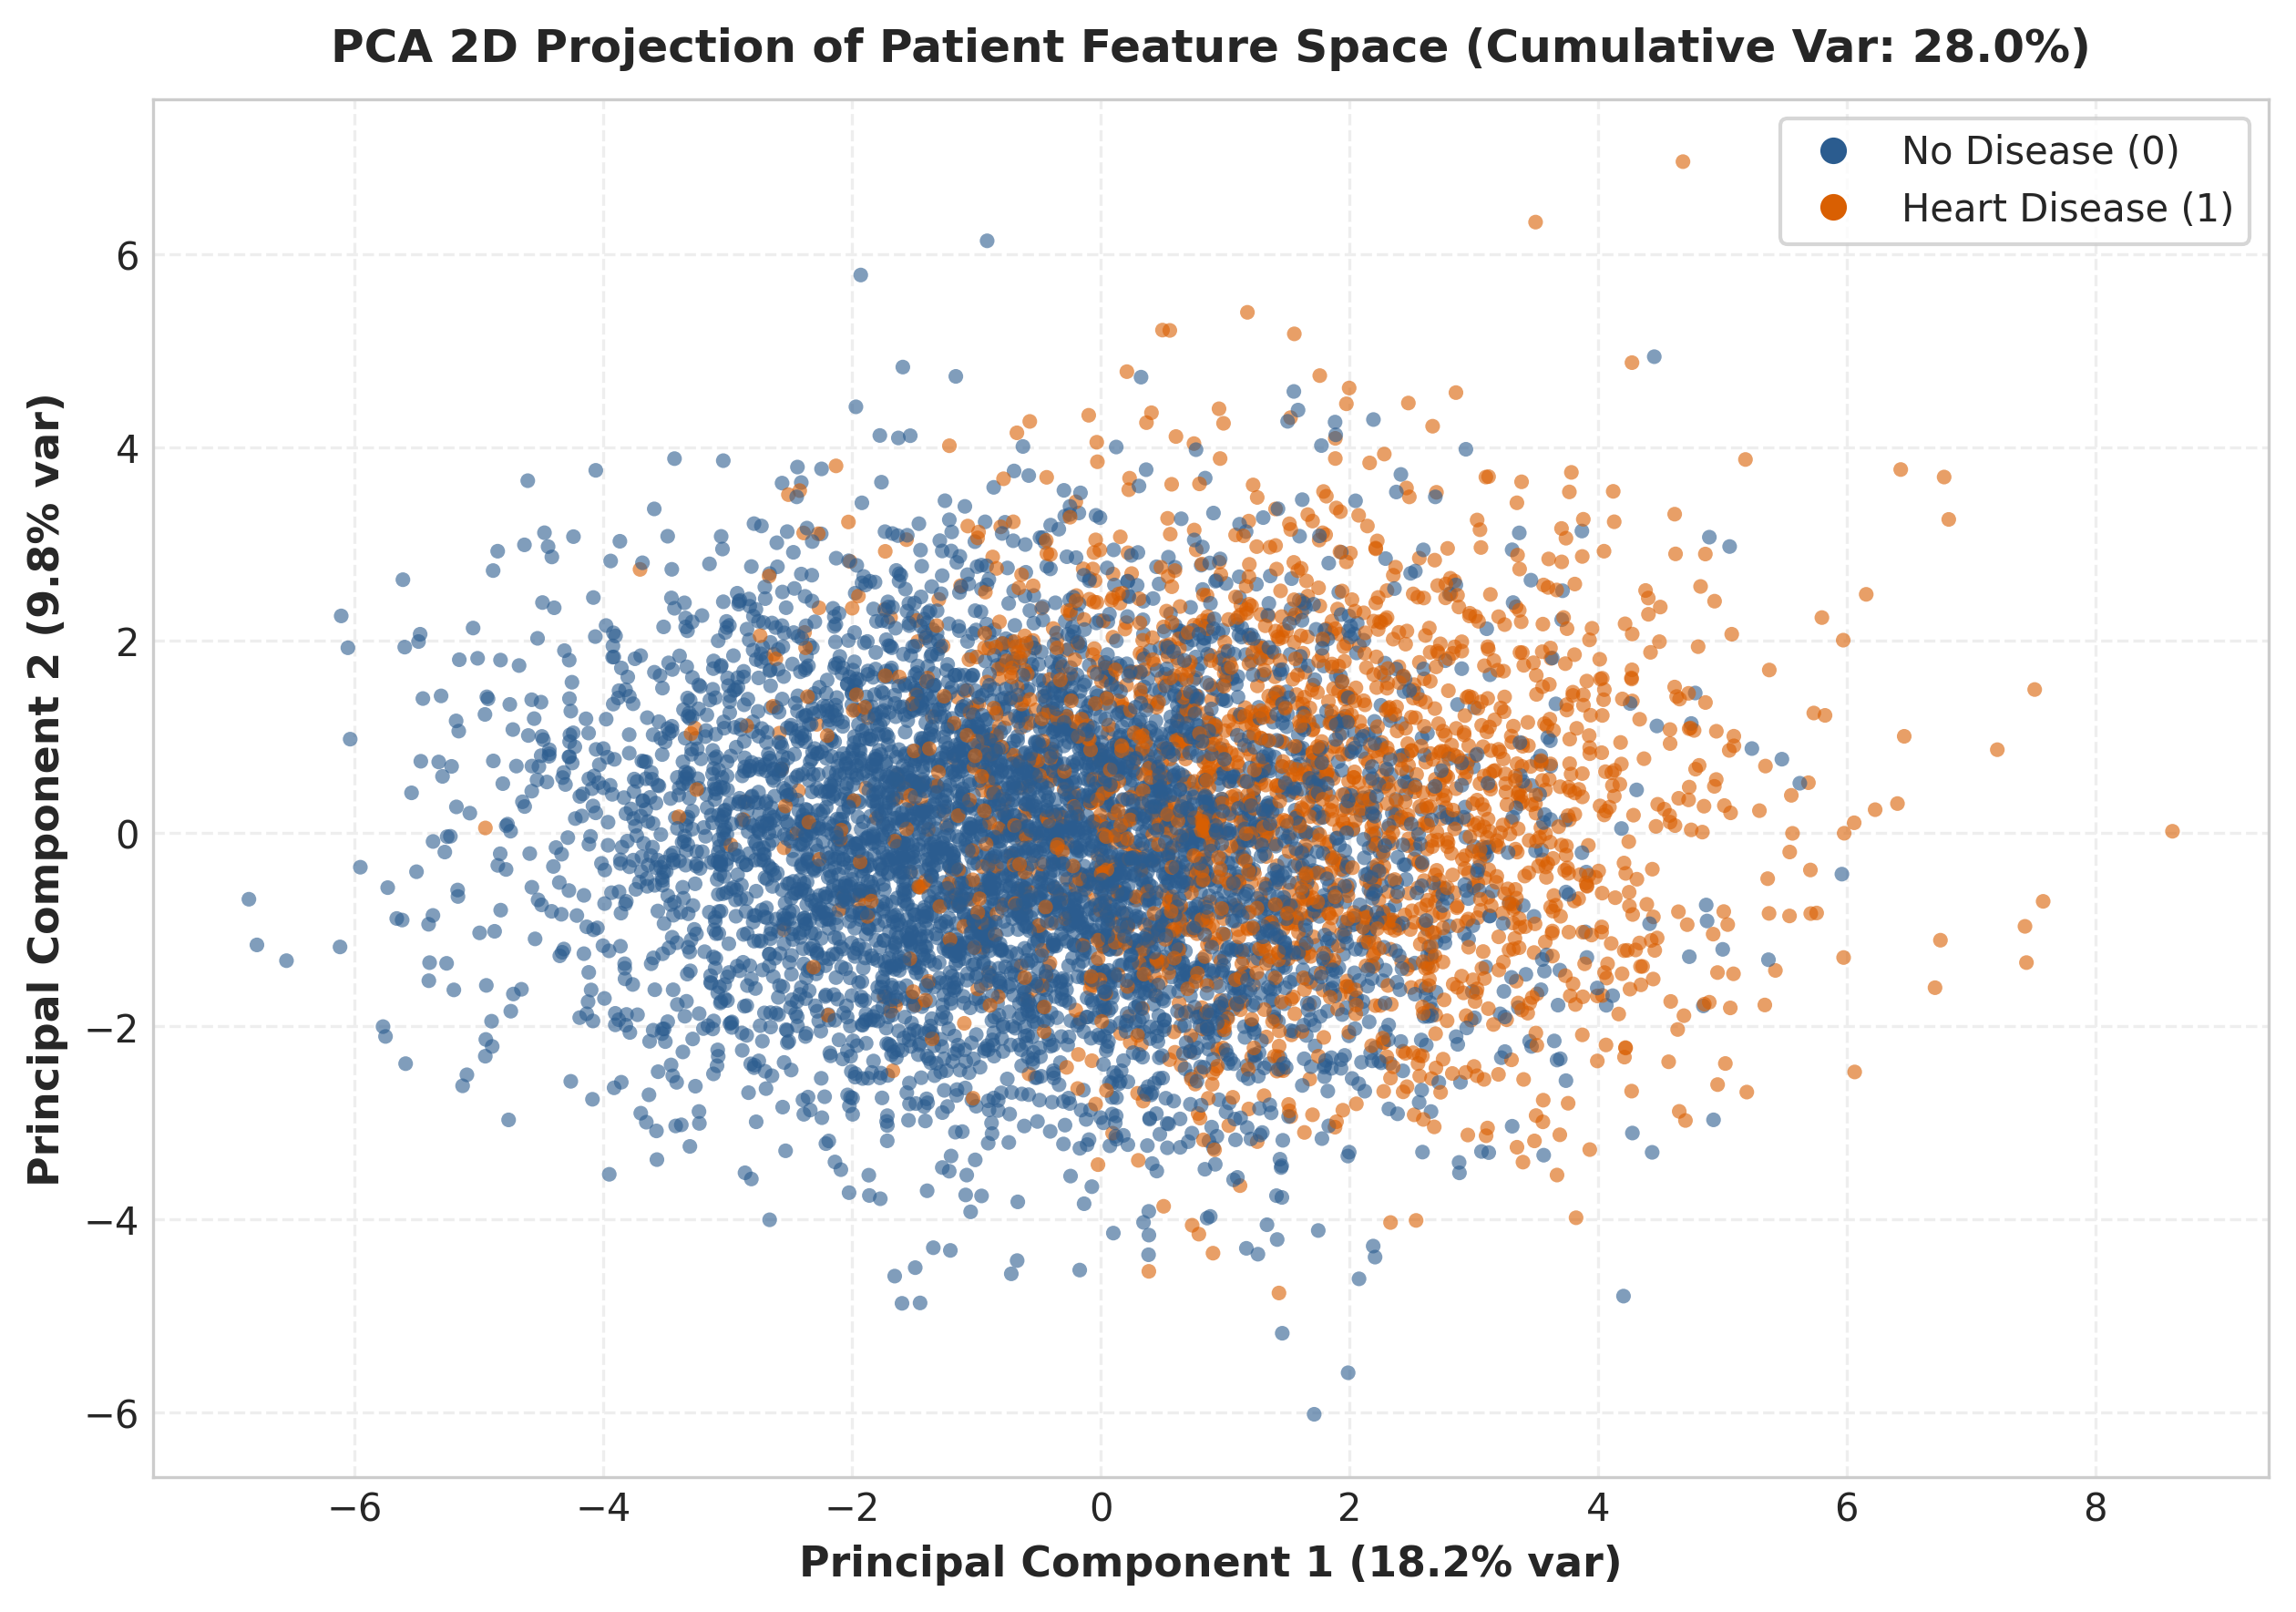
\includegraphics[width=0.85\textwidth]{figures/pca_bivariate_scatter.png}
\caption{Streamlit Application Interactive Data Mining Projection Visual.}
\label{fig:streamlit_flow}
\end{figure}

\section{Application Navigation \& Page Structure}
The dashboard features nine dedicated navigation pages:
\begin{enumerate}
    \item \textbf{Home \& Executive KPI Summary:} Displays high-level KPIs ($9,000$ patients, 25 features, $30.3\%$ prevalence, SVM ROC-AUC $0.9422$), project objectives, and evaluation metrics framework.
    \item \textbf{Dataset Explorer \& Quality Audit:} Interactive filtering by age, target class, search query, categorical pie charts, data dictionary, and summary statistics.
    \item \textbf{EDA Dashboard:} Interactive density inspector, categorical breakdowns, bivariate boxplots, correlation heatmaps, and PCA 2D scatter plots.
    \item \textbf{Statistical Analysis Suite:} Expander views of all 6 hypothesis tests ($\alpha = 0.05$) showing test statistics, raw/FDR $p$-values, effect sizes, plain-language interpretations, and summary tables.
    \item \textbf{Feature Importance Comparison:} Interactive normalized comparison across Mutual Information, Gini Importance, Permutation Importance, and Correlation.
    \item \textbf{Model Benchmark \& Hyperparameters:} Test performance benchmark tables, 5-fold CV hyperparameter badges for all 6 models, ROC curves, and confusion matrix grids.
    \item \textbf{Dynamic Patient Heart Disease Risk Predictor:} Top real-time output card with 7-tier risk scale, visual progress bar, and interactive sliders organized into four importance categories.
    \item \textbf{Key Discoveries \& Findings:} Structured analytical discoveries detailing research questions, methods, results, and data mining implications.
    \item \textbf{About \& Student Contribution Matrix:} Software stack specifications, simulated student contribution matrix, and educational disclaimer.
\end{enumerate}

\section{7-Tier Clinical Risk Stratification Scale}
To translate continuous probability outputs $P(Y=1 \mid \mathbf{x}) \in [0\%, 100\%]$ into actionable medical triage, Page 7 establishes a 7-tier clinical risk scale:

\begin{table}[H]
\centering
\caption{7-Tier Granular Clinical Risk Stratification Scale}
\label{tab:risk_scale}
\small
\begin{tabular}{lcll}
\toprule
\textbf{Risk Tier Label} & \textbf{Probability Range} & \textbf{Badge Color} & \textbf{Clinical Triage Guidance} \\
\midrule
\textbf{ALL OK / NO RISK} & $0.0\% - 14.9\%$ & Emerald Green (\texttt{\#059669}) & Optimal health profile; routine preventive care. \\
\textbf{LOW RISK} & $15.0\% - 29.9\%$ & Light Green (\texttt{\#10B981}) & Biomarkers within normal limits; standard checkups. \\
\textbf{MEDIUM RISK} & $30.0\% - 44.9\%$ & Yellow/Gold (\texttt{\#D97706}) & Mild elevation; lifestyle modifications advised. \\
\textbf{BORDERLINE RISK} & $45.0\% - 54.9\%$ & Orange (\texttt{\#F97316}) & Threshold boundary; secondary screening recommended. \\
\textbf{HIGH RISK} & $55.0\% - 69.9\%$ & High Orange (\texttt{\#EA580C}) & Substantial elevation; clinical evaluation \& lipid therapy. \\
\textbf{VERY HIGH RISK} & $70.0\% - 84.9\%$ & Red (\texttt{\#DC2626}) & High disease likelihood; cardiologist referral. \\
\textbf{DANGER / CRITICAL} & $85.0\% - 100.0\%$ & Dark Red (\texttt{\#991B1B}) & Immediate diagnostic testing (echocardiography). \\
\bottomrule
\end{tabular}
\end{table}

\section{Categorized Interactive Predictor Sliders}
Features on Page 7 are categorized into four color-coded importance tiers:
\begin{itemize}
    \item \textbf{Category 1 (Primary Cardiac Risk Markers):} Max HR, ST Depression, Chest Pain Type, Exercise Angina.
    \item \textbf{Category 2 (Metabolic \& Blood Chemistry):} LDL, HDL, Total Cholesterol, HbA1c, Fasting Blood Sugar, Triglycerides.
    \item \textbf{Category 3 (Hemodynamic Vitals \& Demographics):} Age, Sex, Systolic/Diastolic BP, Resting HR, BMI.
    \item \textbf{Category 4 (Lifestyle \& Behavioral Parameters):} Smoking status, Exercise minutes, Steps, Diet score, Stress, Alcohol, Sleep.
\end{itemize}
As the user drags any slider, the top prediction card updates dynamically in real time.
